\section{Testing and Deployment}
While our planning phase in the first third of the project, we decided to assign responsibilities to team members for different parts of the implementation.
This leads to an independent implementation workflow for every component with the need to put them all together at some time - not only for a final deployment, but also for development of the dependent components ( for instance the pipeline component that use the Provenance API).
To realize a fast development of depenent parts and produce runnable artifacts at any time (as it is usual for a Scrum schedule), we decided to implement a Continuous Integration Workflow based on the commits that was made to the respective Repositories. Each commit was automatically tested (at least whether it is buildable) and, if it was desired, deployed to a Docker or Maven Repository. The current build state of each branch was evaluated immediately after a push so that the code health could be checked by erveryone at any time.
On this way, other parts of the project could include the artifacts by using explicit version tags or \emph{LATEST}-version of the repositories. In the first part of this section, we will describe in detail, how we implemented our CI workflow. In the second part we describe how we used these artifacts for a deployment on AWS\footnote{We used the aws deployment also for our benchmarks (\ref{}).} and which additional adjustments were necessary to get a larger deployment with individual sensor workloads.

\subsection{Continuous Integration \& Delivery}

\paragraph*{Travis CI}
%For every component of our provenance system we created a Github Repository and registered 
%\begin{itemize}
%	\item Pipeline Component \footnote{\url{https://github.com/Krymnos/IDP}}
%	\item Backend\footnote{\url{https://github.com/Krymnos/IDP-backend}}
%	\item Frontend\footnote{\url{https://github.com/Krymnos/IDP-frontend}}
%	\item Provenance API\footnote{\url{https://github.com/Krymnos/Provenance-System-for-IoT}}
%\end{itemize}
%

\begin{figure}[h!]
	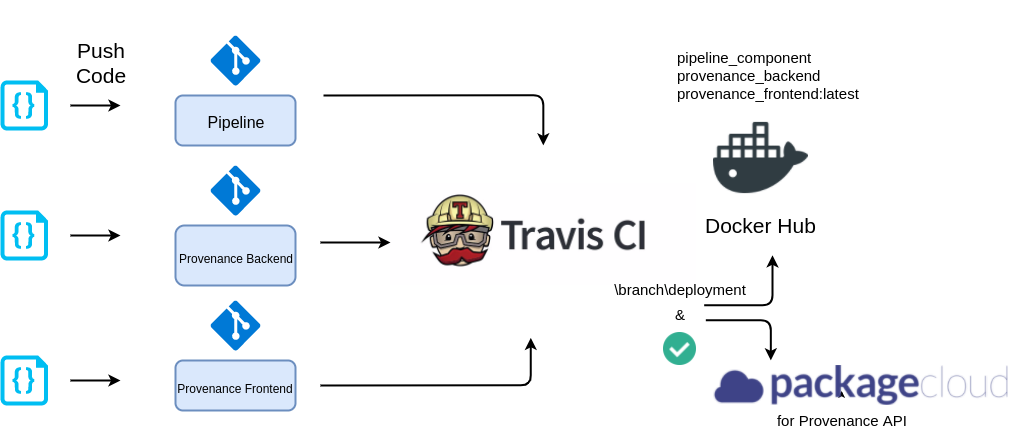
\includegraphics[width=\textwidth]{figures/deployment.png}
	\caption{Deployment Pipeline}
	\label{fig:deployment}
\end{figure}


We used Travis CI\footnote{\url{https://travis-ci.org/Krymnos/IDP}} as Continuous Integration Solution that is free for Open-Source Projects. Travis builds were triggered on changes for every branch of the repository that contains a valid \emph{travis.yaml}.
The testing configuration was set inside of the \emph{travis.yaml} that was present in each repository. Some components needed additional configuration to get builds and tests running. For instance, the Pipeline Component needs the protobuf executables to generate the communication interfaces during a build. After a the compilation is finished, the unit tests of the Pipeline requires a running \emph{Redis}-Database as local storage. All these configurations could be made by the \texttt{before-script} and \texttt{before-install} sections inside the \texttt{travis.yaml} by using the built-in services of travis\footnote{\url{https://docs.travis-ci.com/user/database-setup/}}. As an example, the travis.yaml for the pipeline component can be found in the appendix \ref{lst:pipelineyaml}.
At the same file a \emph{deployment}-section was defined and only executed if the branchname is equal to "deployment". For the components that are delivered as docker builds, the respective docker deployment script was executed \ref{lst:dockerdeploy}, for the Provenance API that is included by the Pipeline Component, the artifacts was pushed to our Maven Repository\footnote{\url{https://packagecloud.io/gerritja/IDP}}. The docker deployment script pushed the docker images to \emph{Docker Hub}-Repository of our project\footnote{\url{https://hub.docker.com/r/cloudproto/}}.

\paragraph*{Docker Images}
We decided to use Docker for the deployment of our components because a docker container runs platform independent, isolated, lightweight and can be interconnect with other services in a very simple way \footnote{\url{https://docs.docker.com/engine/docker-overview/\#docker-engine}}. The Docker engine (in combination wirh docker-compose or Docker Swarm) also supports a good functionality to bring a deployment to a large scale. That suites well to our plans for a fast iterative development and the possibility to test our system on different Topologies.

To deploy our components as Docker images, we added a \emph{Dockerfile} to the Sensor, Pipeline, Backend and Frontend components. A Dockerfile\footnote{\url{https://docs.docker.com/engine/reference/builder/}} contains the instuction that are executed during a build of an image. As well it's defined in a Dockerfile which commands has to be executed on an instantiation of a Container. For the Pipeline Component, for instance, we specified that every instance has a Redis Database running that was started inside the docker container as a local daemon.

To make the Docker Container configurable, we introduced environment variables for the Provenance API and further settings. Also delaying the runtime of the Pipeline Component by setting \texttt{STARTUP\_DELAY}) is possible because we noticed that we had undesired failures at startup because depedent components were not available due a longer instantiaion phase\footnote{for instance, the cassandra database takes usually more time to be available than a lightweight pipeline component}. As an example, the Dockerfile for the pipeline component can be found in the appendix (\ref{lst:pipelinedockerfile}).

\paragraph*{Setup Topologies with docker-compose Files} 
For manual testing of our System and running benchmarks (\ref{chap:Benchmarks}), we defined the individual components and the connection between each other inside a compose file for Docker \footnote{\url{https://docs.docker.com/compose/compose-file}}. The compose files could be therefore used as specification for a deployment with Docker or Docker Swarm.

A simple example that defines a simple pipeline with a workload generator, a gateway and an endpoint can be found in the appendix (\ref{lst:simpletopology}).
The topology can be started on any machine that has Docker installed and a docker-compose and/or docker swarm extension.

\begin{itemize}
	\item command for docker swarm:\texttt{docker stack deploy -f <composefile> <stackname> }
	\item command for docker-compose:\texttt{docker-compose -f <composefile> up} 
\end{itemize}


\subsection{Docker Swarm on AWS}
Due to the machine independability of docker containers we're able to deploy our topology locally but also along distributed machines.
As \emph{docker-compose} is sufficient for a local deployment on one node, \emph{Docker Swarm} is used to distribute the orchestration of the components over multiple machines which are organized within a cluster and running on \emph{swarm mode} \footnote{\url{https://docs.docker.com/engine/swarm/key-concepts/}}.

To setup such a cluster on AWS we used a predefined Cluster template for \emph{AWS Cloud Formation}\footnote{\url{https://editions-us-east-1.s3.amazonaws.com/aws/stable/Docker.tmpl}} that is provisioned by Docker \footnote{\url{https://docs.docker.com/docker-for-aws}}. A detailed readme, how a topology can be deployed is available on the IDP repository on \texttt{deployment/howto.md}\footnote{\url{https://github.com/Krymnos/IDP/blob/master/deployment/howto.md}}

\subsubsection*{Scaling of Sensors/Workload}
For our project we got circa 6 GB of real sensor data with measurements of a power grid. The data contains folders for every day in a year. Each folder contains usually 10 data items (csv files), each is representing a sensor. We wanted to be able to test more than 10 sensors in our deployment.

\paragraph*{data preparation}
We modified the origin strucure of the sensor data in a way that one folder contains all files to simulate many more sensors for only one day.
The workload generator that sends the data to our pipeline components determines a sensor id by the filename (e.g. \texttt{31400010000000000.csv}). We had to rename the files due to the issue of having many duplicate filenames. We numbered the files consecutively to get increasing sensor ids (from 31400010000000000 to 31400010000003473) so that we're able to simulate up to 3474 unique sensors\footnote{\url{https://s3.console.aws.amazon.com/s3/buckets/provenancesensordata/data/oneday} note: the access to the sensordata is restricted due to privacy reasons}.

\paragraph*{data inclusion}
To have the ability to run a sensor container completely without external sensor data, we stored a small dataset (few megabytes) inside the sensor container-image.
For our plans to scale sensors with unqique sensor data it was obviously not an option to put 6 GB into a docker image. Also the creation of thousands of sensor images (with few megabytes for a unique sensor) makes no sense.
Therefore, we stored the sensor data to a \emph{Amazon S3} Bucket and implemented a docker image for the sensor that has the skill to mount bucket inside the local filesystem of the container\footnote{We forked an existing base image to add this functionality \url{https://github.com/serioja90/docker-goofys}}. An example that can be used inside a docker compose file can be found in the appendix \ref{sensors3}.

This approach worked fine for a local deployment on one node by using \emph{docker-compose}. Unfortunately, we had to realize, that this image doesn't work on \emph{Docker Swarm}, because the priviliged execution of the docker container is mandatory to mount the S3 Bucket inside. The priviliged mode is supported by \emph{docker-compose} but not by \emph{Docker Swarm}\footnote{a discussion/open issue about that can be found here: https://github.com/moby/moby/issues/24862}.
To get a working access to the S3 bucket, we defined an external \emph{docker volume}\footnote{\url{https://docs.docker.com/storage/volumes}} in the compose file in combination with a docker plugin that links the S3 bucket with the docker volume \footnote{https://hub.docker.com/r/rexray/s3fs}.

\paragraph*{scalable sensor groups}
At this point, we were able to mount the complete sensor data on a efficient way. We still had the problem, that a definition of unique sensors was only possible by adding a service entry for every single sensor to the compose file, because the sensor was explicitely expecting the datapath to the measurement file.
Docker provides a scale command \footnote{\url{https://docs.docker.com/compose/reference/scale/}} that can be used to scale up services of indentical instances. To define sensor groups of unique sensor by using this command we implemented another service for sensor-id coordination. This service implements a simple counter that gives the current id as an response of a REST-Request and increments it.
We modified the sensor code in a way, that a sensor calls the REST endpoint of the coordinator and adds the received id to the basepath of the sensordata folder on the mounted data\footnote{The implementation of the coordinator and the modifications in the sensor implementation can be found here: \url{https://gitlab.tubit.tu-berlin.de/gerrit.janssen/smemu}}. 

The appendix contains a simple example of mounting the S3 bucket and the id coordinator approach\ref{lst:sensorsscale}


\subsubsection*{Deployment of the complete stack}
We created different versions of compose files with different Topologies and all components. The files can be found in the IDP-Repository at: \texttt{compose-files}\footnote{https://github.com/Krymnos/IDP/tree/master/compose\_files}. In this folder exists also a readme that describes, how to instatiate a topology locally  with \emph{docker-compose}\footnote{ Some compose files containing special constraints for aws, for instance to schedule nodes in different availability zones.}.

Figure \ref{fig:finaldeployment} shows a the general scheme for a deployment on AWS.

\begin{figure}[h!]
	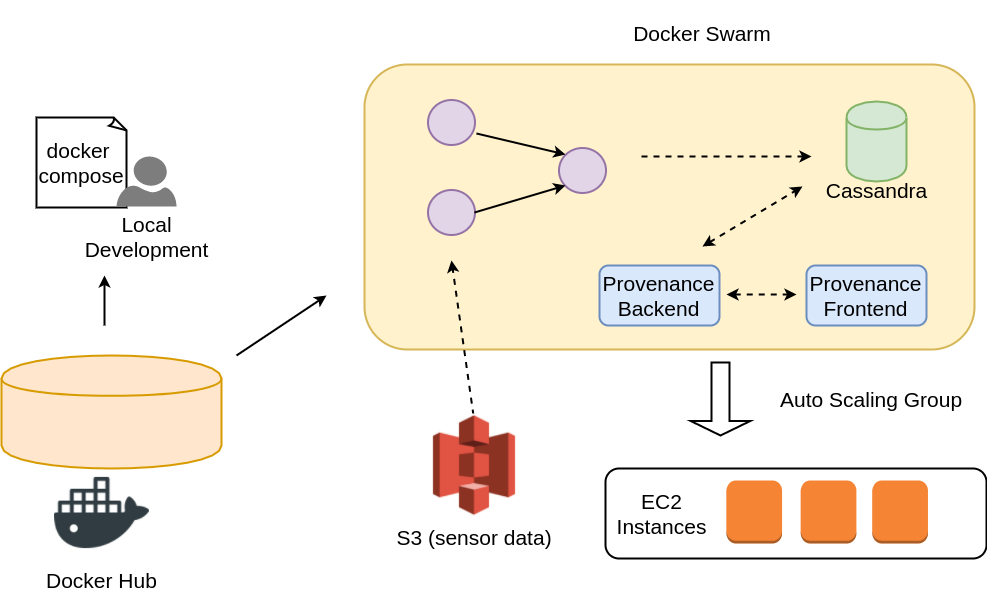
\includegraphics[width=\textwidth]{figures/deployment2.png}
	\caption{deployment scheme of the complete stack on AWS}
	\label{fig:finaldeployment}
\end{figure}